De manera similar queremos el precio de una bomba de calor por unidad de
potencia eléctrica máxima (compresor). Aunque generalmente resulta más
accesible la potencia calorífica, así que para los casos donde no hemos
encontrado la potencia máxima del compresor, hemos asumido un COP (Coefficient
Of Performance) mínimo de 3.4. Los datos \footnote{de
	\url{https://www.climamarket.eu/}} son recogidos en el cuadro
\ref{tab:heat_pump_data}, y la regresión lineal mostrada en
\ref{fig:heat_pump_regression}

\begin{table}[htbp]
	\centering
	\begin{tabular}{llrrr}
		\toprule
		Marca      & Modelo         & Potencia máxima del compresor [W] & Precio [\euro] & \euro / W \\
		\midrule
		Mitsubishi & PUD-SWM80YAA   & 1764.71                           & 2600           & 1.47      \\
		Mitsubishi & PUD-SWM100YAA  & 2352.94                           & 3500           & 1.49      \\
		Mitsubishi & PUD-SHWM80VAA  & 1764.71                           & 3700           & 2.10      \\
		Mitsubishi & PUD-SWM120YAA  & 2941.18                           & 4000           & 1.36      \\
		Mitsubishi & PUD-SHWM100YAA & 2352.94                           & 4400           & 1.87      \\
		Mitsubishi & PUD-SHWM120YAA & 2941.18                           & 4700           & 1.60      \\
		Haier      & AU052FYCRA(HW) & 1470.59                           & 2200           & 1.50      \\
		Johnson    & AURUM80M       & 2441.18                           & 2700           & 1.11      \\
		Johnson    & AURUM100M      & 3529.41                           & 3200           & 0.91      \\
		Panasonic  & WH-MDC05J3E5   & 1470.59                           & 3400           & 2.31      \\
		Haier      & AU112FYCRA(HW) & 3235.29                           & 3500           & 1.08      \\
		Lg         & HM071MR.U44    & 2058.82                           & 3500           & 1.70      \\
		Johnson    & AURUM-AT90M    & 2647.06                           & 3700           & 1.40      \\
		Johnson    & AURUM160M      & 4705.88                           & 3900           & 0.83      \\
		Panasonic  & WH-MDC07J3E5   & 2058.82                           & 3900           & 1.89      \\
		Lg         & HM051MR.U44    & 1617.65                           & 4000           & 2.47      \\
		Lg         & HM091MR.U44    & 2647.06                           & 4100           & 1.55      \\
		Panasonic  & WH-MDC09J3E5   & 2647.06                           & 5000           & 1.89      \\
		Lg         & HM121MR.U34    & 3529.41                           & 5200           & 1.47      \\
		Panasonic  & WH-MDC12H6E5   & 3529.41                           & 5400           & 1.53      \\
		Lg         & HM123MR.U34    & 3529.41                           & 5400           & 1.53      \\
		Lg         & HM141MR.U34    & 4117.65                           & 5700           & 1.38      \\
		Daikin     & EBLA09D3V3     & 2735.29                           & 6000           & 2.19      \\
		Lg         & HM143MR.U34    & 4117.65                           & 6200           & 1.51      \\
		Lg         & HM161MR.U34    & 4705.88                           & 6500           & 1.38      \\
		Daikin     & EBLA11D3V3     & 3411.76                           & 6600           & 1.93      \\
		Panasonic  & WH-MDC16H6E5   & 4705.88                           & 6624           & 1.41      \\
		Lg         & HM163MR.U34    & 4705.88                           & 6840           & 1.45      \\
		Daikin     & EBLA14D3V3     & 3529.41                           & 7300           & 2.07      \\
		Daikin     & EBLA16D3V3     & 4705.88                           & 8200           & 1.74      \\
		Johnson    & AURUM200T      & 5882.35                           & 5600           & 0.95      \\
		Lg         & HM121HF.UB60   & 3529.41                           & 7500           & 2.13      \\
		Daikin     & EKHBRD016ADY17 & 4705.88                           & 14000          & 2.98      \\
		Daikin     & EKHBRD011ADV17 & 3235.29                           & 10700          & 3.31      \\
		Daikin     & EKHBRD011ADY17 & 3235.29                           & 11600          & 3.59      \\
		Daikin     & EKHBRD016ADV17 & 4705.88                           & 13000          & 2.76      \\
		Daikin     & EKHBRD014ADV17 & 4117.65                           & 11900          & 2.89      \\
		\bottomrule
	\end{tabular}
	\caption{Modelos de bombas de calor.}
	\label{tab:heat_pump_data}
\end{table}


\begin{figure}[h] \centering
	\centering
	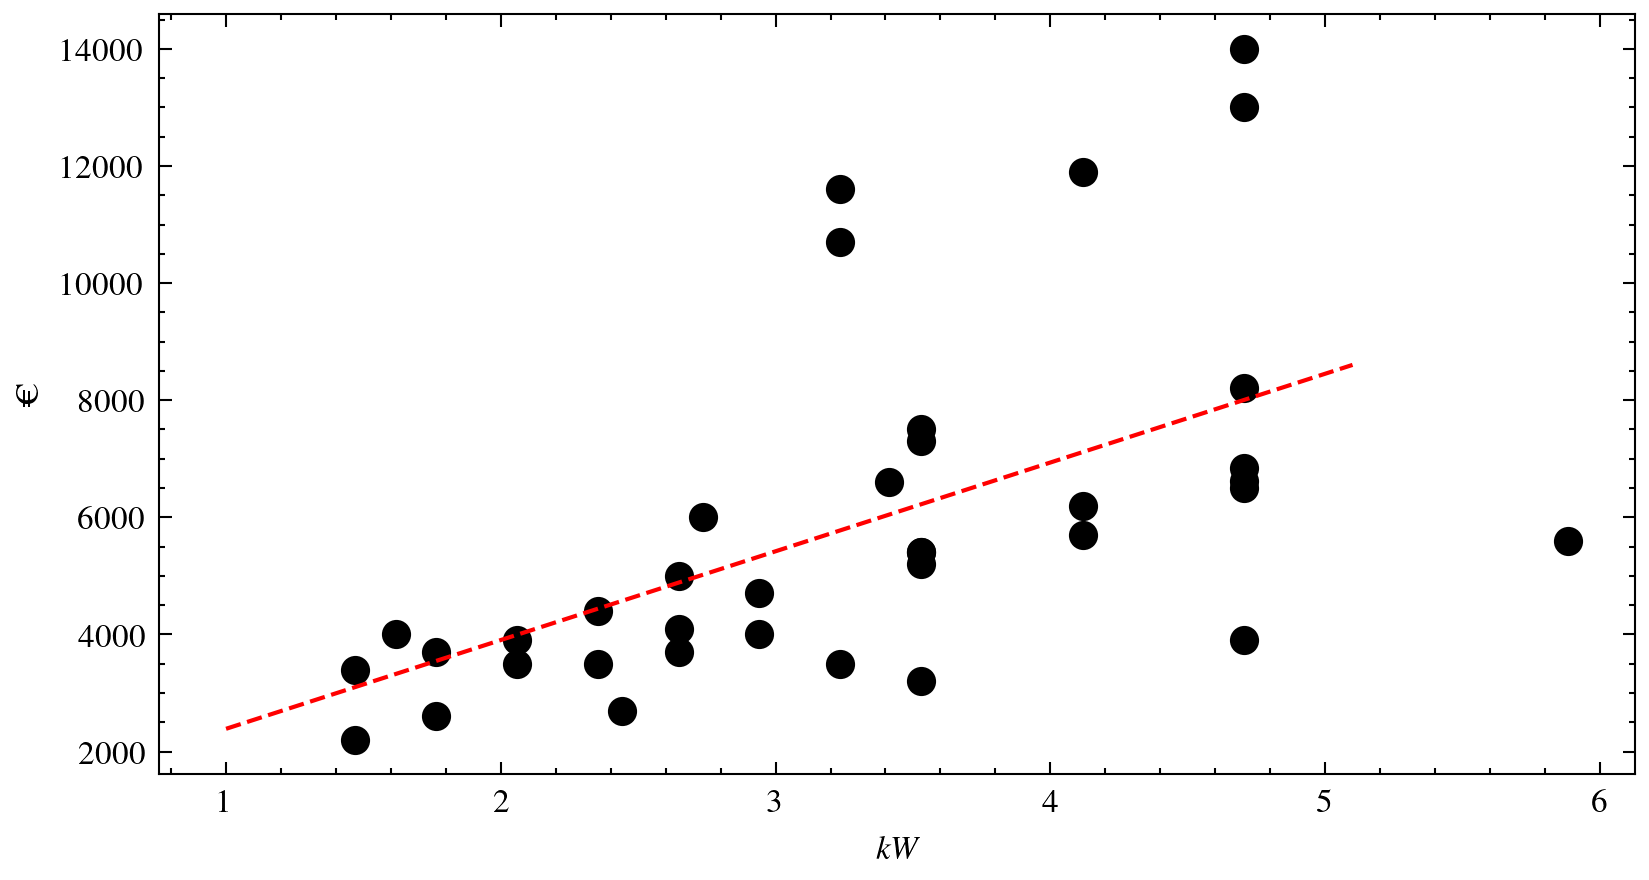
\includegraphics[width=1\textwidth]{./capitulos/adquisicion_de_datos/images/heat_pump_regression.png}
	\caption{Ajuste lineal de precios para bombas de calor.}
	\label{fig:heat_pump_regression}
\end{figure}


La expresión para el coste por unidad de potencia es la siguiente:

\begin{equation}
	\text{coste\_bomba\_calor} \left[\frac{\text{\euro}}{kW}\right] = 871.93 + 1783.40 \cdot P_{bomba_{max}}
\end{equation}

donde $P_{bomba_{max}}$ es la potencia máxima del compresor de la bomba de calor.
